\documentclass[conference,final]{IEEEtran}

\usepackage[utf8]{inputenc}
\usepackage{graphicx}
\usepackage{url}
\usepackage{float}
\usepackage{times}    
\usepackage{listings}   
\usepackage{times}     
\usepackage{paralist}    
\usepackage{wrapfig}    
\usepackage[small,it]{caption}
\usepackage{multirow}
\usepackage{ifpdf}    
\usepackage{subfig} 
\usepackage{color}
\usepackage{natbib}   
\usepackage{pdfsync}
\usepackage{fancyvrb}

\newenvironment{shortlist}{
	\vspace*{-0.85em}
  \begin{itemize}
  \setlength{\itemsep}{-0.3em}
}{
  \end{itemize}
	\vspace*{-0.6em}
}

\DefineShortVerb{\|}
\DefineVerbatimEnvironment{mycode}{Verbatim}
{
  label=Code Example,
  fontsize=\small,
  frame=single,
% framerule=1pt,
  framesep=1em,
  numbers=right,  %numbers=right,
  numbersep=2pt,
  gobble=2,
  numberblanklines=false
}

% \title{pplication-level Interoperability between Clouds and Grids}
% \title{SAGA-MapReduce: Providing Infrastructure Independence and
%   Cloud-Grid Interoperability}
\title{Programming Abstractions for Data Intensive Computing on Clouds and Grids}

\author{Michael Miceli$^{12}$, Chris Miceli$^{12}$, Shantenu
  Jha$^{123}$, Hartmut Kaiser$^{1}$, Andre Merzky$^{1}$, \\
  \small{\emph{$^{1}$Center for Computation \& Technology, Louisiana
      State University, USA}}\\
  \small{\emph{$^{2}$Department of Computer Science, Louisiana State
      University, USA}}\\
  \small{\emph{$^{3}$e-Science Institute, Edinburgh, UK}}\\
}

\newif\ifdraft
%\drafttrue
\ifdraft
\newcommand{\amnote}[1]{ {\textcolor{magenta} { ***AM: #1c }}}
\newcommand{\jhanote}[1]{ {\textcolor{red} { ***SJ: #1 }}}
\newcommand{\michaelnote}[1]{ {\textcolor{blue} { ***MM: #1 }}}
\else
\newcommand{\amnote}[1]{}
\newcommand{\jhanote}[1]{}
\newcommand{\michaelnote}[1]{ {\textcolor{blue} { ***MM: #1 }}}
\fi

\newcommand{\sagamapreduce }[1]{SAGA-MapReduce }
\newcommand{\tc }[1]{$T_c$}
\begin{document}

\maketitle

\begin{abstract}
  MapReduce has emerged as an important data-parallel programming
  model -- for data-intensive computing for clouds and grids. However
  most if not all implementations of MapReduce are coupled to a
  specific infrastructure.  SAGA is a high-level programming interface
  which provides the ability to create distributed applications in an
  infrastructure independent way. In this paper, we show how MapReduce
  has been implemented using SAGA and demonstrate its interoperability
  across different platforms -- distributed Grids, Clouds and
  Cloud-like infrastructure. Using data-sets of size upto 10GB, we
  provide detailed performance analysis of the SAGA-MapReduce
  implementation.  We discuss the advantages of programmatically
  creating MapReduce to be infrastructure independent, for example,
  the ability to control the distribution and placement of compute
  enables the user to decide where to place the workers (with data in
  mind), and thus keep data network transfter costs low --- both time
  and cost....
\end{abstract}

% \keywords{programming models for clouds, computing in the cloud,
%   interoperability}

\section*{Structure aka Grand Plan}\jhanote{this section will not
  stay}

% Why do we need Programming Abstractions for data intensive computing
% on Clouds and Grids

% \begin{enumerate}
% \item  Infrastructure Independent
%    The plethora of Cloud Systems (have grossman figure)!
%    Ain't no difference from Grids.

% \item Application level programming pattens and data-access remains
% invariant on differernt infrastructure, thus decompose
% according to the logic/patterns

% \item  Need for different and novel Programming Models:\\
%   Cloud PM need to have control over data and compute placement

% \begin{itemize}
%  \item for perfomance (obvious)
%  \item cost of computing!!
%        same thing, same performance done different can cost very differently
%        hence need to be able to control placement of compute and work
% \end{itemize}

% Grids: Regular perfomance issues
% \end{enumerate}

The *RIGHT* Abstraction will provide 1. infrastructure independence,
2. support for decomposing along application patterns, 3. support for
different and novel programming models. Most if not all of the three
features /criteria. SAGA is an important useful approach.  To
demonstrate/provide irrefutable evidence of the above, we:

\begin{itemize}
\item {\bf Develop SAGA-MapReduce }

  \begin{itemize}
  \item Implement SAGA-MapReduce which enables us to control chunk
    size, location of compute
  \item Profile SAGA-MapReduce and compare it to Yahoo's MapReduce
    (Hadoop) on both HDFS and KFS.
  \end{itemize}

\item {\bf Deploy and test it on Grids}
  \begin{itemize}
  \item Local vs Distributed Compute Resources
  \item Compute launched as regular jobs (GRAM)
  \item local/Regular file systems on different machines
  \item regular advert service for coordination
  \end{itemize}

For each case (where applicable):
  \begin{itemize}
  \item We repeat distributed runs on upto 3 distributed systems
    (LONI)
  \item Understand how performance of SAGA-MapReduce changes with i)
    number of workers and ii) data-set sizes and iii) chunk sizes
  \end{itemize}

\item {\bf Deploy and test it on Cloud-like Systems} Underlying fabric
  is Grids, but we use distributed file-systems (KFS, HDFS) and
  big-table for coordination.
\item {\bf SAGA-MapReduce on Cloud}
  \begin{itemize}
  \item Establish SAME SAGA-MapReduce. Distinguish semantics of same
    function call (show API similarity)
  \item The Three Cloud Systems we play with are:
    \begin{itemize}
    \item AWS
    \item Nimbus
    \item Eucalyptus (GumboCloud -- howzatt!!)
    \end{itemize}
  \item Do tests for 1,2..10 Workers with 1,2..10 GB
  \item Analagous to Grids/LONI We want to do half workers on AWS and
    half on Nimbus or some combination of the three systems thereof
  \end{itemize}
\end{itemize}

Voila! Once we've done all this, we've established SAGA as an
infrastructure independent and good performing abstraction for
data-intensive application as outlined in the opening.

\section{Introduction} 

The case for effective programming abstractions and patterns is not
new in computer science.  Coupled with the heterogeneity and evolution
of large-scale distributed systems, the fundamentally distributed
nature of data, and the exponential increase of data -- collection,
processing, storing, it can be argued that there is a greater premium
than ever before on abstractions at multiple levels.

% The case for effective programming abstractions and patterns is not
% new in computer science. But it can be argued that the heterogeneity
% of distributed systems, and their continuous and rapid evolution
% places greater premium on abstractions at the multiple levels than
% before.  Coupled with the evolution of large-scale distributed systems
% and the fundamentally distributed nature of data, is the exponential
% increase of data -- collection, processing, storing. 

With the force-of-industry behind the development (and not just the
hype) of Clouds, although they are a nascent infrastructure, their
impact can not be ignored.  Specifically, with the emergence of Clouds
as important distributed computing infrastructure, we need
abstractions that can support the dominant programming models for
Clouds. Issues of scale aside, ideally the transition from existing
(primarily Grids) programming models and styles, must be as seamless
and as least distruptive as possible, else it risks engendering
technical and political horror stories as by Globus -- which became an
unfortunate and disastrous by-word for everything wrong with the
complexity of Grids.

Inevitably, the unified concept of a Cloud is evolving into different
flavours and implementations on the ground. For example, there are
already multiple implementations of Google's BigTable, such as Hbase
etc.  There is bound to be a continued proliferation of such
Cloud-like infrastructure; this is reminiscent of the plethora of grid
middleware distributions.

As {\it application-level} programming and data-access patterns remain
essentially invariant on differerent infrastructure, the ability to
support application specific data-access patterns is both useful and
important~\cite{dpa-paper}.  Having said that, there are
infrastructure specific -- technical and policy, features that need to
be addressed. For example, Amazon, the archetypical Cloud System has a
well-defined cost model for data transfer across {\it its}
network. Hence, Programming Models for Clouds must be cognizant of the
requirement to programmatically control data and compute placement.
It is not that traditional Grids applications do not have this
interesting requirement, but that such explicit support is required
only for very large-scale and high-performing applications in
traditional Grid environments. In contrast, for most Cloud
applications it is required in order to ensure basic cost
minimization, i.e., the same computational task can be priced very
differently for possibly the same performance.  These factors and
trends place a critical importance on effective programming
abstractions for data-intensive applications for both Clouds and Grids.
%-- which is the primary motivation of this work.
Any {\it effective} abstraction will be cognizant and provide most, if
not all of the above features. The primary aim of this work is to
establish that SAGA is an {\it effective} abstraction that can support
different programming models and is usable on traditional (Grids) and
emerging (Clouds) distributed infrastructure.  Our approach is to
begin with a well understood data-parallel programming model
(MapReduce), implement it using a standard programming interface --
the Simple API for Grid Applications (SAGA).  SAGA has been
demonstrated to support distributed HPC programming models and
applications effectively; it is an important aim of this work to
verify if SAGA has the expressiveness to implement data-parallel
programming and is capable of supporting acceptable levels of
performance (as compared with native implementations of
MapReduce). After this conceptual validation, our aim is to use the
{\it same} implementation of MapReduce on a range of Cloud systems,
and test for inter-operability between different flavours of Clouds as
well as between Clouds and Grids.


% \jhanote{it is important to compare gene-search using MapReduce and a
%   simple straighforward application; similarly a multiple alignment
%   excercise without using All-Pairs..}

\section{SAGA}
SAGA~\cite{saga-core} is a high level API that provides a simple,
standard and uniform interface for the most commonly required
distributed functionality.  SAGA can be used to encode grid
applications~\cite{saga_escience07_short, saga_tg08}, tool-kits to manage
distributed applications as well as implement abstractions that
support commonly occurring programming, access and usage patterns.

\begin{figure}[t]
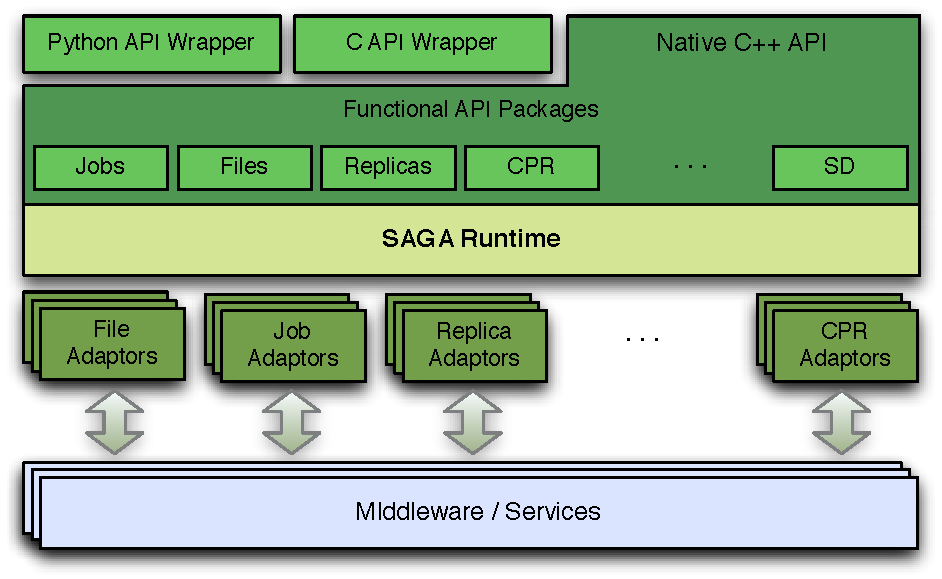
\includegraphics[scale=0.5]{saga-figure02.pdf}
\caption{In addition to the programmer's interface,
  the other important components of the landscape are the SAGA engine,
  and functional adaptors.}
\label{saga_figure}
\end{figure}

Fig.~\ref{saga_figure} provide a view of the SAGA landscape, and the
main functional areas that SAGA provides a standardized interface
to. Based upon an analysis of more than twenty applications, the most
commonly required functionality involve job submission across
different distributed platforms, support for file access and transfer,
as well as logical file support. Less common, but equally critical
wherever they were required, is the support for Checkpoint and
Recovery (CPR) and Service Discovery (SD).  The API is written in C++
with Python, C and Java language support. The {\it engine} is the main
library, which provides dynamic support for run-time environment
decision making through loading relevant adaptors. We will not discuss
details of SAGA here, as there exist several well documented
sources~\cite{saga_url}.

%  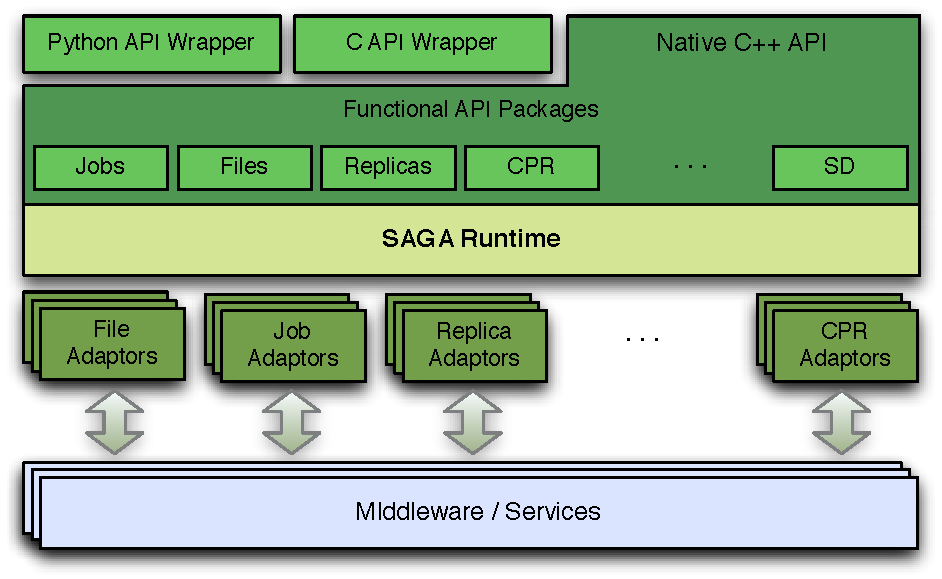
\includegraphics[width=0.44\textwidth]{saga-figure02.pdf}


%  In addition, the aim of
% this paper is to show (validate) that SAGA is sufficiently complete
% and has a high-level interface to support these programming
% abstractions.

% Figure~\ref{fig:data_intensive_app_saga} illustrates the software
% architecture of the implementation, highlighting the different
% abstraction levels that allow the reuse of most of the system for both
% algorithms and for different genomic applications.

\jhanote{Include only if there is space: Some of the programming
  models that are common to both data-intensive application and
  Cloud-based computing, where there is an explicit cost-model for
  data-movement, is to develop general heurisitcs on how we handle
  common considerations such as when to move the data to the machine
  or when to process it locally.}

\section{Patterns for Data-Intensive Computing: MapReduce and
  All-Pairs}

In this paper we will demonstrate the use of SAGA in implementing well
known programming patterns for data intensive computing.
Specifically, we have implemented MapReduce and the All-Pairs
patterns, and have used their implementations in SAGA to to solve
commonly encountered genomic tasks.  We have also developed real
scientific applications using these implementations of these patterns:
multiple sequence alignment can be orchestrated using the
SAGA-All-pairs implementation, and genome searching can be implemented
using SAGA-MapReduce.

The implementation of these patterns encapsulates details such as
latency hiding, performance and other variables (such as cluster
sizes, and queue sizes).  The user should be able to easily add a few
function calls without necessarily having to worry about many of the
non-functional considerations often required by applications using
distributed environments.  In general, SAGA can shield the application
developer from many of these considerations, while still providing the
sophisticated end-user the ability to control these performance and
cost critical/determining factors.

\jhanote{Only if space permits: We will discuss other performance
  issues that arise when implementing abstractions specific for
  data-intensive computing.  A grid application's design should not
  focus on the bandwidth of the network, the dispatch latency, the
  number of machines available, and data reliability.  Even something
  as simple as process size can be a tough challenge to optimize.  If
  a job is too small, then network traffic becomes a bottleneck and
  the design is inefficient.  If a job is too large, it is difficult
  to tell when it is hanging or still computing.  Also, if another job
  with a higher priority takes a machine over, the application will be
  waiting on jobs longer.  The main point of this paper is to show how
  a flexible, extensible implementation of programming data-intensive
  abstractions using SAGA can shield the application developer from
  many of these considerations, while still providing the
  sophisticated end-user the ability to control these performance and
  cost critical/determining factors.}

{\bf MapReduce: } MapReduce is a programming framework developed by
Google for running data-intensive processes over a large cluster of
commodity machines.  The main idea is to provide an easy interface for
users to solve a specific domain of problem with grids without having
the client worry about the semantics of the grid, for example,
dispatch latency, machine failure, data distribution, and network
bandwidth.  All of these are problems that could make some naïve
implementations on a grid slower than serial implementations.  When
using a MapReduce implementation, the programmer interacts with only
two functions: map and reduce.  The map function will go through the
datasets and create a map of data to some type of output.

A map is a datatype in computer science that relates one object to
another, i.e. a name to a phone number.  The reduce function will go
through all of the maps and combine them to produce another output.
The de facto example is word count.  Say, one has a large set of
documents and he wants to find how many of each word is present in all
the documents.  The map function would go through each document and
for every word produce a map from the document to a list of 1’s.  An
example for the word “cat” may look like this cat $\Rightarrow$ 1, 1,
1, 1, 1.  Then, the reduce function will add up the 1’s to produce a
final output, i.e. cat $\Rightarrow$ 5.  At first this framework may
seem limiting, but this is in part what makes it so successful.  Its
structure is is very easily parallelized.  Also, there have been a
large number of distinct applications written using it, and its
popularity has been steadily increasing.  This shows that the
framework is well suited for solving data-intensive problems.

One feature worth noting in MapReduce is that the ultimate dataset is
not on one machine, it is partitioned on multiple machines located
throughout the grid. Google uses their distributed file system (Google
File System) to keep track of where each file is located.
Alternatively, they store MapReduce results in Bigtable.  % We will
% attempt to imitate this using our implementation of MapReduce over
% HDFS.  Also, we will use HBase for communication between jobs.

MapReduce~\cite{mapreduce-paper} is a programming framework which
supports applications which operate on very large data sets on
clusters of computers.  MapReduce relies on a number of capabilities
of the underlying system, most related to file operations.  Others are 
related to process/data allocation.  The Google File System, and other
distributed file systems, provide the relevant capabilities, such as atomic
file renames.  Implementations of MapReduce on these distributed file systems
are free to focus on implementing the data-flow pipeline, which is the
algorithmic core of the MapReduce framework.

{\bf SAGA-MapReduce Implementation:} We have recently implemented
MapReduce in SAGA, targeting general purpose Grid systems, where the
system capabilities required by MapReduce are usually not natively
supported; instead, a general purpose grid provides a much larger set
of lower level operations.  Some semantics, such as again the atomic
file rename, is provided by the SAGA API layer, others, such as
data/compute allocation are not.  Our implementation is thus required
to interleave the core logic with explicit instructions on where
processes are to be scheduled.  Note that some of the required
capabilities can be provided by higher level grid services -- those
are, however, often not standardized, and often not available on
general purpose Grids.

The advantage of this approach is obviously that our implementation is
no longer bound to run on a system providing the appropriate semantics
originally required by MapReduce, but is portable to other, more
generic systems as well.  The drawback of the approach is obvious as
well: our implementation is relatively more complex, as it needs to
add semantic system capabilities at some level or the other, and it is
inherently slower, as it is for these capabilities very difficult or
near impossible to obtain system level performance on application
level.  Critically however, none of these complexities are transferred
to the end-user, and they remain hidden within the framework. Also
many of these are due to the early-stages of SAGA and incomplete
features implementated, and not a fundamental limitation of the design
or concept of the interface or programming models that it supports.

The SAGA based implementation of MapReduce has been developed with the
following goals in mind:

\begin{itemize}
\item Provide a generic MapReduce framework allowing easy
  adaptation to the users concrete Mapreduce algorithm
\item Ensure portability of the users MapReduce application over a
  broad range of Grids and Clouds, filesystems and architectures
\item Allow fine control over the number of workers, and the
  placement of data and computation, ensuring to move the work to the
  data instead of having to move the data to the work
\end{itemize}

The overall architecture of the SAGA-MapReduce implementation is shown
in Fig.~\ref{saga-mapreduce_controlflow}. This simple interface
provides the complete functionality needed by any MapReduce algorithm,
while hiding the more complex functionality, such as chunking of the
input, sorting of the intermediate results, launching and coordinating
the map and reduce workers, etc. as implemented by the framework.  The
application consists of two independent processes, a master and worker
processes. The master process is responsible for:

\begin{figure}[t]
      \centering
          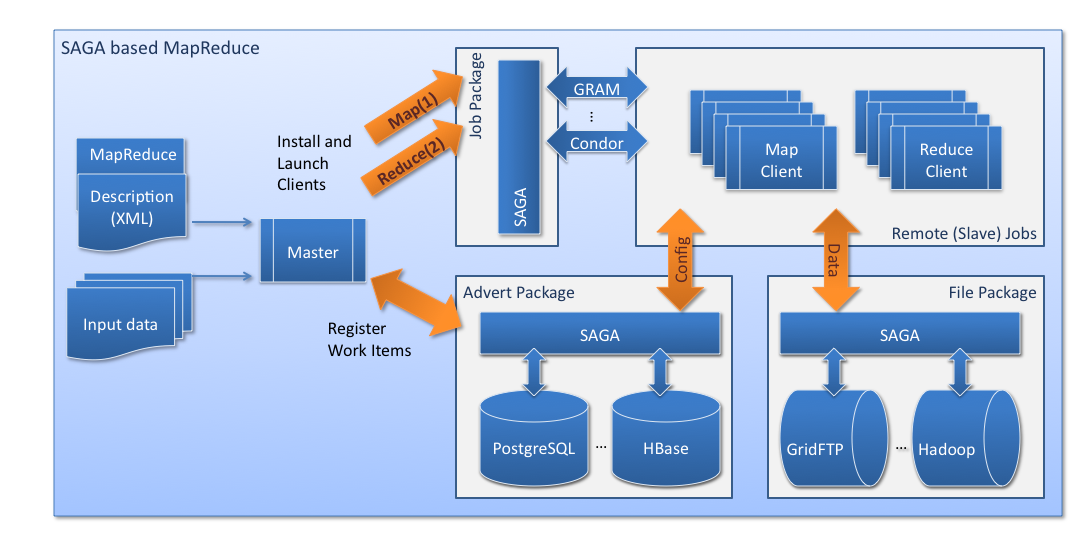
\includegraphics[width=0.4\textwidth]{saga-mapreduce_controlflow.png}
          \caption{High-level control flow diagram for
            SAGA-MapReduce. SAGA uses a master-worker paradigm to
            implement the MapReduce pattern. The diagram shows that
            there are several different infrastructure options to a
            SAGA based application; in particular for MapReduce there
            are ``file coordination'' options -- Hadoop versus
            GridFTP, and for coordination Hbase or a PostgreSQL
            database could be used. There are performance issues with
            the number (and thus size) of chunks and the number of
            resources over which these chunks are distributed.
            \jhanote{I think there should be something between the
              Map(1) and the Reduce(2) phases.. something that comes
              back to the Master, non?}}
      \label{saga-mapreduce_controlflow}
\end{figure}

\begin{itemize}
\item Launching all workers for the map and reduce steps as described
  in a configuration file provided by the user (defining the number of
  workers, the systems/batch queues to use for job execution, the
  input data to use and the output filenames towrite the results to)
\item Coordinating all the executed workers, this includes the
  chunking of the data, assigning the input data to the workers of the
  map step, sorting the intermediate data produced by the map step and
  passing the names of the sorted output to
  the workers of the reduce step, and collecting the generated outputs
  from the reduce steps.
\item Relaunching single worker instances in case of failures,
\end{itemize}

The master process is readily available to the user and needs no
modification for different MapReduce algorithms to execute.  The
worker processes get assigned work either from the map or the reduce
step. The functionality for the different steps have to be provided by
the user, which means the user has to write 2 C++ functions
implementing the required MapReduce algorithm.
Fig.\ref{src:saga-mapreduce} shows a very simple example of a
MapReduce application allowing to count the word frequencies in the
input data set. The user provided functions |map| (line 14) and
|reduce| (line 25) are invoked by the MapReduce framework during the
map and reduce steps. The framework provides the URL of the input data
chunk file to the |map| function, which should call the function
|emitIntermediate| for each of the generated output key/value pairs
(here the word and it's count, i.e. '1', see line 19). During the
reduce step, after the data has been sorted, this output data is
passed to the |reduce| function. The framework passes the key and a
list of all data items which have been associated with this key during
the map step. The reduce step is expected to call the |emit| function
(see line 34) for each of the final output elements (here: the word
and its overall count). All key/value pairs that are passed to |emit|
will be combined by the framework into a single output file.

\begin{figure}[!ht]
 \begin{center}
  \begin{mycode}[label=SAGA MapReduce Word Count Algorithm]
  // Counting words using SAGA-MapReduce
  using namespace std;
  using namespace boost;

  class CountWords 
    : public MapReduceBase<CountWords> {
  public:
    CountWords(int argc, char *argv[]) 
      : MapReduceBase<CountWords>(argc, argv) 
    {}

    // Separate input into words
    // Input:  url of input chunk (chk)
    // Output: separated words and associated 
    //         data (here: '1')
    void map(saga::url chk) {
      using namespace boost::iostreams;
      stream<saga_file_device> in(chk.str());
      string elem;
      while(in >> elem) 
        emitIntermediate(elem, "1");
    } 

    // Count words
    // Input:  word to count (key)
    //         list of associated data items
    // Output: words and their count
    void reduce(string const& key, 
      vector<string> const& values) {
      typedef vector<string>::iterator iter;

      int result = 0;
      iter end = values.end();
      for (iter it = values.begin(); 
           it != end; ++it) {
        result += lexical_cast<int>(*it);
      }
      emit(key, lexical_cast<string>(result));
    }
  };
  \end{mycode}
  \caption{\label{src:saga-mapreduce} Counting word frequencies using
    SAGA-MapReduce. This is the worker-side code.}
 \end{center}
\end{figure}

As shown in Fig.~\ref{saga-mapreduce_controlflow} both, the master and
the worker processes use the SAGA-API as an abstract interface to the
used infrastructure, making the application portable between different
architectures and systems. The worker processes are launched using the
SAGA job package, allowing to launch the jobs either locally, using
Globus/GRAM, Amazon Web Services, or on a Condor pool. The
communication between the master and the worker processes is ensured
by using the SAGA advert package, abstracting an information database
in a platform independent way. All file transfer operations are based
on the SAGA file package, providing a broad range of different file
systems and transfer protocols, such as local file systems,
Globus/GridFTP, KFS, and HDFS.

\begin{figure}[t]
      \centering
          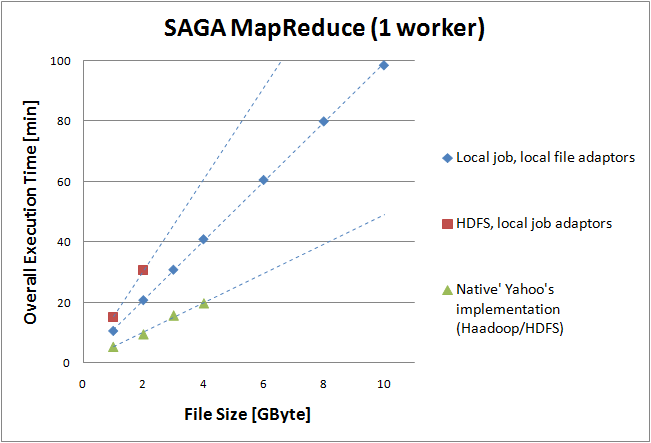
\includegraphics[width=0.25\textwidth]{saga_mapreduce_1worker.png}
          \caption{Performance figures for SAGA-MapReduce, using one
            worker (and local to the master). %  and thus not
%             distributed, but localised to a single machine,
%             \jhanote{could the master and worker not be on different
%               machines? if so, should we call this ``local'' or
%               ``distributed''?}, 
            Case I corresponds to the use of the local file system on
            the Linux clusters we use, while Case II corresponds to
            the use of HDFS on the cluster.  It is interesting to note
            that as the data-set sizes get larger HDFS starts
            outperforming local file systems.  We attribute this to
            the use of caching and other advanced features in HDFS
            which proove to be useful even though it is not being used
            in a distributed fashion. We compare \sagamapreduce to
            Yahoo's MapReduce implementation. % The three different
%             scenarios considered are (i) all infrastructure is local
%             and thus SAGA's local adapters are invoked, (ii) local job
%             adaptors are used, but the hadoop file-system (HDFS) is
%             used, (iii) Yahoo's mapreduce. 
            Yahoo's mapreduce takes less time than \sagamapreduce
            implementations, by about a factor of 2. This is not
            surprising, as SAGA based implementations have not been
            optimised, for example, \sagamapreduce is not
            multi-threaded}
      \label{saga_mapreduce_1worker.png}
\end{figure}

\begin{figure}[t]
      \centering
          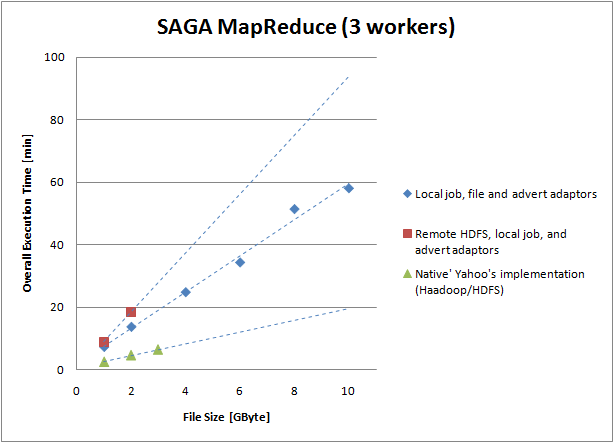
\includegraphics[width=0.25\textwidth]{saga_mapreduce_3workers.png}
          \caption{stuff will come..}
      \label{saga_mapreduce_3workers.png}
\end{figure}

The Master process creates partitions of data (referred to as chunking, analagous to Google's MapReduce), so the data-set does not have to be
on one machine and can be distributed; this is an important
mechanism to avoid limitations in network bandwidth and data distribution.
These files could then be recognized by a distributed file systems
such as Hadoop File System.

% There are a few implementations of MapReduce, most notably Google's and
% Hadoop's.  These are what our implementation is based on.  It is able
% to handle most of the problems associated with grid applications.  We use
% the idea of a master/slave type framework.  The programmer would compile
% different slave applications for every different type of machine he 
% would expect to encounter in the grid.  The slave application is
% where the map and reduce functions are.  Then the master will handle
% submitting these jobs on other machines as well as keeping track of
% the state of the machines -- idle, done, or failed.  This allows for
% easy running of an application using large girds that have frequent
% machine failures.  Our MapReduce also handles data distribution in the
% same manner Google does, 
  % Although, our current implementation is
% written to avoid excessive network bandwidth, it does not change
% depending on current network availability.

% \subsubsection{Gene Searching}

% Gene searching is an important part of biology.  \michaelnote{I'm sure
%   Shantenu knows more about why gene searching is an important part of
%   biology than I do!}

% MapReduce can easily be used to find certain gene fragments in a large
% gene file.  The mapping function looks through its input and if it
% finds the sequence - or something close - it will then produce a map
% of a file to a position in the file where the fragment started.  The
% reduce will then take every map and append the results.  The is good
% for searching large datasets, because it is easily done through
% MapReduce, ensuring network reliability, and parallelization.

{\bf All-Pairs: } As the name suggests, All-Pairs involve comparing
every element in a set to every element in another set.  Such a
pattern is pervasive and finds utility in many domains -- including
testing the validity of an algorithm, or finding an anomaly in a
configuration.  For example, the accepted method for testing the
strength of a facial recognition algorithm is to use All-pairs
testing.  This creates a similarity matrix, and because it is known
which images are the same person, the matrix can show the accuracy of
the algorithm.

% All-pairs testing is a useful tool in testing the reliability of a
% produce - an algorithm, software, hardware, \ldots.  This is because
% many times one small difference in a configuration can show
% incompatibilities.  However, testing is not the only field in which
% All-pairs is useful.  Anywhere every element from one set has to be
% compared to every element from another set, All-pairs can help.  This
% is the main goal of All-pairs to ensure that every combination of
% pairings from two sets is tested.

{\bf SAGA All-Pairs Implementation: } SAGA All-pairs implementation is
very similar to \sagamapreduce implementation.  The main difference is
in the way jobs are ran and how the data are stored.  In
\sagamapreduce the final data is stored on many machines -- if there
is a distributed filesystem available, whereas SAGA All-pairs uses the
database to also store information about the job.  We decided to do
this because all data must be available to be useful. SAGA All-Pairs
abstraction is implemented using the Hadoop File System and using
gridftp to not only show that SAGA allows for many different
configurations, but also to see how these different configurations
behave. We have also used a distributed data-store -- specifically
Hbase (Yahoo's implementation of BigTable) in lieu of the traditional
Advert Service to store the end-results.

% We could have used a distributed file system such as HDFS, but we
% felt that the output was not large enough to constitute this.  This
% is due to the fact that - although the data is relatively large -
% the result should usually be a real number representing the distance
% of two genes.

{\it Multiple Sequence Alignment Using All-Pairs:} All-Pairs is
essentially a computational pattern and not an application in of
itself. An important problem in Bioinformatics -- Multiple Sequence
Alignment (MSA), can be reformulated to use All-Pairs pattern. It uses
a comparison matrix as a reference to compare many fragment genes to
many base genes.  Each fragment is compared to every base gene to find
the smallest distance -- maximum overlap.  Distance is computed by
summing up the amount of similarity between each nucleotide of the
fragment to each one in the base.  This is done starting at every
point possible on the base. The result of the smallest distance is
then stored for that fragment using a database management system --
Hbase, Bigtable, Postgresql, \ldots.


\section{Interfacing SAGA to Cloud-like Infrastructure: The role of
  Adaptors}

\jhanote{talk about Hadoop and Bigtable, KFS}

As alluded to, there is a proliferation of Clouds and Cloud-like
systems, but it is important to remember that Clouds are not well
defined systems, or ``what constitutes or does not consitute a Cloud''
is not universally agreed upon.  However there are several aspects and
attributes of Cloud systems that are generally agreed
upon~\cite{buyya_hpcc}. A minimal set of these attributes can be
considered the use of virtualized machines, support for distributed
file and structured data storage.  Here we will by necessity limit our
discussion to two type of distributed file-systems (HDFS and KFS) and
two types of distributed structured-data store (Bigtable and Hbase)
that we have developed SAGA adaptors for, and over which
\sagamapreduce and SAGA All-Pairs works seamlessly.

% Extended and additional attributes could include AppEngine style
% environments. 
% http://www.gridbus.org/papers/hpcc2008_keynote_cloudcomputing.pdf

% We used hadoop as a metadata storage, work still needs to be done to
% see how well SAGA-MapReduce is at accessing elements as part of
% mapping

% Data intensive applications require large amounts
% of data to be available at run-time in a reliable and efficient
% manner. 

{\it HDFS and KFS: }The Hadoop Distributed File System (HDFS) is a
distributed parallel fault tolerant application that handles the
details of spreading data across multiple machines in a traditional
hierarchical file organization.  % It has been highly successful and is
% currently used by Yahoo!, Facebook, and the New York Times to name a
% few.  HDFS also handles replication and striping of data for
% fault-tolerance.  
Implemented in Java, HDFS is designed to run on commodity hardware
while providing scalability and optimizations for large files.  The
file system works by having one or two namenodes, masters, and many
rack-aware datanodes, slaves.  All data requests go through the
namenode that uses block operations on each data node to properly
assemble the data for the requesting application.  The goal of
replication and rack-awareness is to improve reliability and data
retrieval time based on locality.  In data intensive applications,
these qualities are essential. \jhanote{Michael, can you put in a few
  words about KFS here please?}

{\it Bigtable and HBase:} Bigtable~\cite{bigtable_small} is a specific
type of database system created by Google to have better control over
scalability and performance than other databases.  It is very flexible
and has many advantages over normal databases.  The main difference is
that it is meant to store extremely large datasets, into the
petabytes, over thousands of machines.  Another advantage is the
ability to be accessed through MapReduce.  Since MapReduce is
inherently very well parallelized, accessing Bigtable is very
efficient.  Due to the success of Bigtable, HBase was developed by as
an open source alternative to Bigtable for use with Hadoop.  Both
HBase and Bigtable split up large tables and replicate them over many
machines to avoid node failure.  Also, since the data are partitioned
accessing it does not create a large strain on the network bandwidth.

There exist many other implementations of both distributed
file-systems (such as Sector) and of distributed data-store (such as
Cassandra and Hybertable); for the most part they are variants on the
same theme technically but different language and performance criteria
optimizations.  Hypertable is an open-source implementation of
Bigtable; Cassandra is another Bigtable clone but eschews an explicit
coordinator (Bigtable's Chubby, HBase's HMaster, Hypertable's
Hyperspace) for a P2P/DHT approach for data distribution and location
and for availability.  In the near future we will be providing
adaptors for Sector~\footnote{http://sector.sourceforge.net/} and
Cassandra~\footnote{http://code.google.com/p/the-cassandra-project/}
As testimony to the power of SAGA, the ability to create the relevant
adaptors in a lightweight fashion and thus extend applications to new
systems with minimal overhead is an important design feature and a
significant requirement so as to be an effective programming
abstraction layer.

% \jhanote{repeat the motivation for using both ``native'' and
%   non-native infrastructure dependence}

\section{SAGA as an interface to Clouds and Grids}

% \jhanote{Describe the native implementation of mapreduce\\
%   essentially explain how this is yahoo's mapreduce: hadoop + hdfs}

% We are going to use the default advert service of SAGA (SQL) to 
% communicate between jobs as well as store information about 
% individual jobs.

% In this experiment we are going to use the Hbase advert service 
% provided by SAGA to determine how it compares to the default advert 
% service, i.e. speed, and latency.

% We are going to mimic Google's MapReduce, which uses the Google File
% System (GFS) to store intermediate and final results.  They also store
% metadata about the grid with Bigtable.  Since we do not have GFS or
% Bigtable available to use, we are going to use the Hadoop File system
% (HDFS) and HBase to store the metadata similar to what Yahoo! uses.
% We will call this the native implementation of MapReduce.

Experiments are:
\begin{enumerate}
\item \sagamapreduce` when both compute (workers) and
  data-distribution is local. The number of workers vary from 1 to 10,
  and the data-set sizes varying from 1 to 10GB. Here we will also compare
  \sagamapreduce` with native MapReduce (using HBase and Hadoop)
\item \sagamapreduce` when workers are locally computed, but using a distributed file system (HDFS); the number of workers varies from 1 to 4
% upto 3 workers (upto a data-set size of 10GB).
\item The same as Experiment 2, but using a different file system
  (KFS) and the number of workers vary from 1 to 10
\item \sagamapreduce` using distributed compute (workers) and distributed file-system (KFS)
\item Distributed compute (workers) but using local file-systems (using gridftp for transfer)
\end{enumerate}

We have also distinguished between SAGA All-Pairs using Advert Service
versus using Hbase for data-store, but due to space constraints we
will report results of the All-Pairs experiments elsewhere.

\subsection{SAGA-MapReduce on Grids}

\begin{figure}[t]
  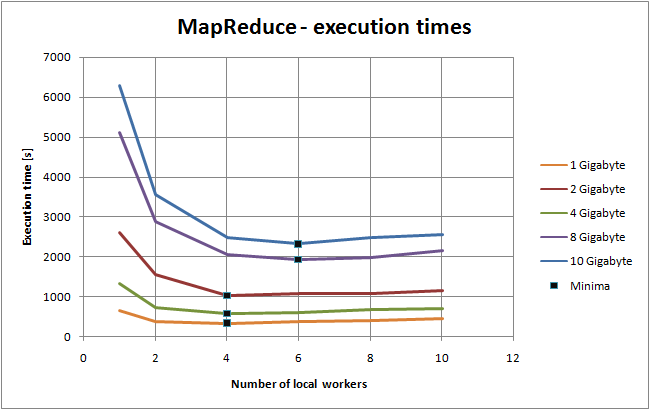
\includegraphics[width=0.4\textwidth]{MapReduce_local_executiontime.png}
\caption{Plots showing how the \tc for different data-set sizes
  (1-10GB) varies with the number of workers employed.
  Larger the data-set creater the advantage of more workers. For
  example, As the data-set size increases, the number..}
\label{grids1}
\end{figure}

\begin{figure}[t]
  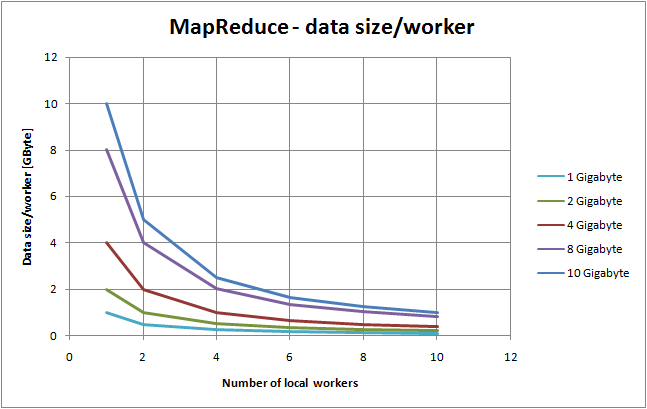
\includegraphics[width=0.4\textwidth]{MapReduce_local_datasizeperworker.png}
\caption{Stuff will go here}
\label{grids2}
\end{figure}

\begin{figure}[t]
  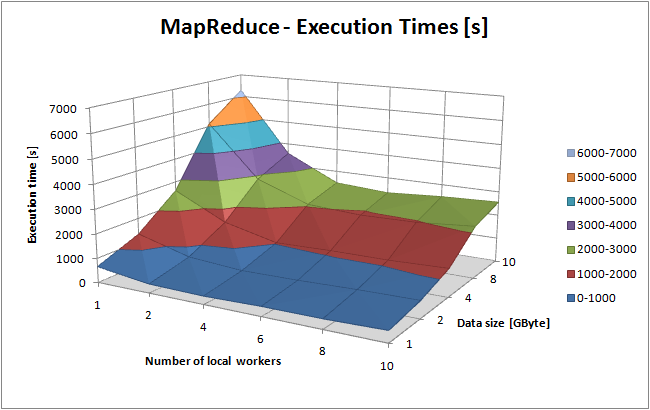
\includegraphics[width=0.4\textwidth]{MapReduce_local_executiontime_3d.png}
\caption{Stuff will go here too}
\label{grids3}
\end{figure}

Experiments 1 and 3; Figures~\ref{grids1}, \ref{grids2}, \ref{grids3}

% \begin{figure}[t]  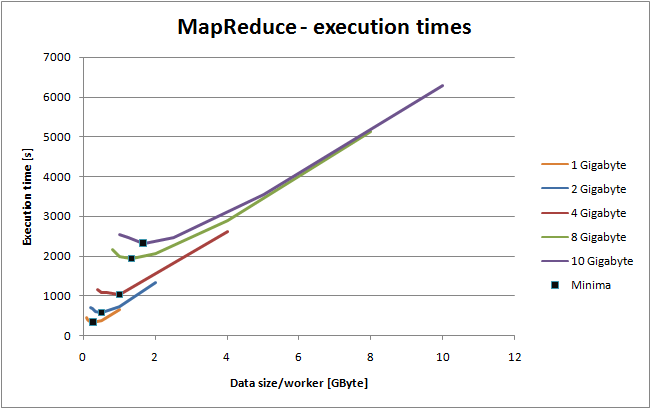
\includegraphics[width=0.4\textwidth]{MapReduce_local_executiontimeperworkerdatasize.png}\label{4}
% \end{figure}


% \begin{figure}[t]
% 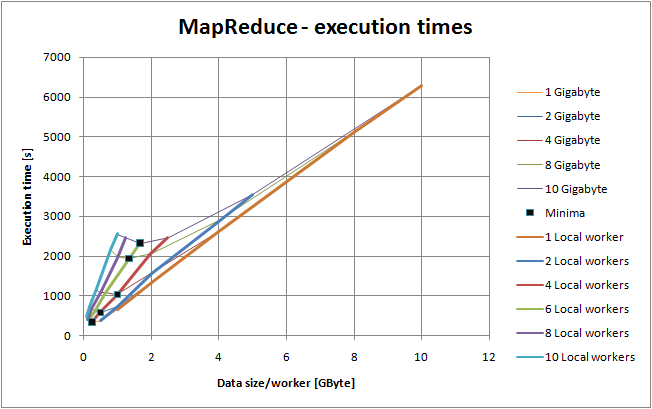
\includegraphics[width=0.4\textwidth]{MapReduce_local_executiontimeworkersdatasize2.png}
% \label{5}
% \end{figure}

\subsection{SAGA-MapReduce on Cloud-like infrastructure}

Experiment 2 and 4; Figures ~\ref{saga_mapreduce_1worker.png},
~\ref{saga_mapreduce_3workers.png}

\subsection{SAGA-MapReduce on Clouds}

\begin{itemize}
\item  The Three Cloud Systems we play with are:
\begin{itemize}
\item AWS
\item Nimbus
\item Eucalyptus (GumboCloud -- howzatt!!)
\end{itemize}
Now compare performance of 1,2..10 Workers with 1,2..10 GB
\item Analagous to Grids/LONI We want to do half workers on AWS and half 
on Nimbus or some combination of the three systems thereof
\end{itemize}

\begin{figure}[!ht]
 \begin{center}
  \begin{mycode}[label=SAGA Job Launch via GRAM gatekeeper]
   {// finds a GRAM gatekeeper
    saga::job::service js;
    saga::job::description jd;
    jd.set_attribute(``Executable'', ``/tmp/my_prog'');
    //translate job description to RSL
    saga:job::job j = js.create_job(jd);
    //submit RSL to gatekeeper, and obtain job handle
    j.run():
    // watch handle until job is finished
    j.wait();
   } 
  \end{mycode}
  \caption{\label{gramjob}Job launch via Gram }
 \end{center}
\end{figure}


\begin{figure}[!ht]
 \begin{center}
  \begin{mycode}[label=SAGA create a VM instance on Eucalyptus]
   {// create a VM instance on Eucalyptus
    saga::job::service js;
    saga::job::description jd;
    jd.set_attribute(``Executable'', ``/tmp/my_prog'');
    //translate job description to ssh command
    saga:job::job j = js.create_job(jd);
    //run the ssh command on the VM
    j.run():
    // watch command until done
    j.wait();
   } 
  \end{mycode}
  \caption{\label{vmjob} Job launch via VM}
 \end{center}
\end{figure}


\section{Conclusion}

We have also shown the importance and power of patterns in
data-intensive computing. Patterns capture a dominant and recurring
computational mode; by providing explicit support for such patterns,
end-users and domain scientists can reformulate their scientific
problems/applications so as to use these patterns. For example, we
have shown how traditional bioinfomatics applications such as Multiple
Sequence Alignment and Gene Search can be implemented using the
All-Pairs and MapReduce patterns. This provides further motivation for
abstractions at multiple-levels -- to support basic functionality but
also data-intensive patterns.



% \subsection*{SAGA Based MapReduce}
% Performance figures when using the Advert service -- on one machine,
% on >1 machine, finding the bottleneck

% \jhanote{These figures can then be used to justify some of the 
%   development efforts proposed in OMIISAGA-2}

\section{Acknowledgments}

Important funding for SAGA specification and development has been
provided by the UK EPSRC grant number GR/D0766171/1.  SJ also
acknowledges the e-Science Institute, Edinburgh for supporting the
research theme, ``Distributed Programming Abstractions''.  This work
would not have been possible without the efforts and support of other
members of the SAGA team. This work has also been made possible thanks
to the internal resources of the Center for Computation \& Technology
(CCT) at Louisiana State University and computer resources provided by
LONI. Michael Miceli was supported by a Google Summer of Code grant.
\bibliographystyle{plain} \bibliography{saga_data_intensive}
\end{document}

%As we shall show, SAGA is an important useful approach.
% and hence need to be able to control placement of compute and work
% same performance done different 

%\begin{enumerate}
% \item Application level programming pattens and data-access remains
%   invariant on differernt infrastructure, thus decompose according to
%   the logic/patterns

% \item  Infrastructure Independent
%    The plethora of Cloud Systems (have grossman figure)!
%    Ain't no difference from Grids.

% \item Programming Models for Clouds having interesting
%   requirements:\\
%   Cloud PM need to have control over data and compute placement

% \begin{itemize}
%  \item for perfomance (obvious)
%  \item cost of computing!!
%        same thing, same performance done different can cost very differently
%        hence need to be able to control placement of compute and work
% \end{itemize}
% Grids: Regular perfomance issues
% \end{enumerate}

% \begin{figure}[t]
%       \centering
%           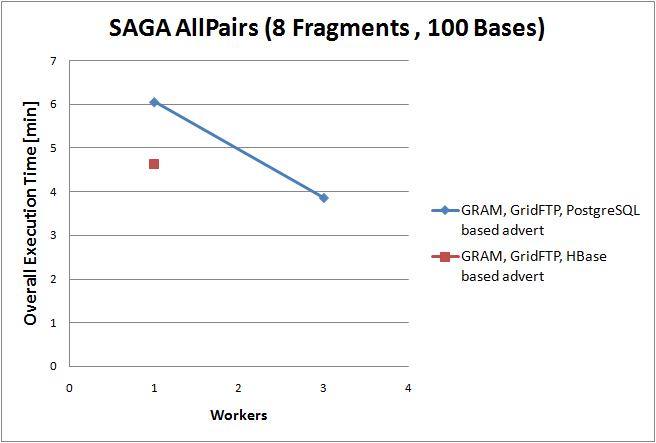
\includegraphics[width=0.8\textwidth]{saga_allpairs.png}
%           \caption{}
%       \label{sagaallpairs}
% \end{figure}

% \begin{figure}[t]
%       \centering
%          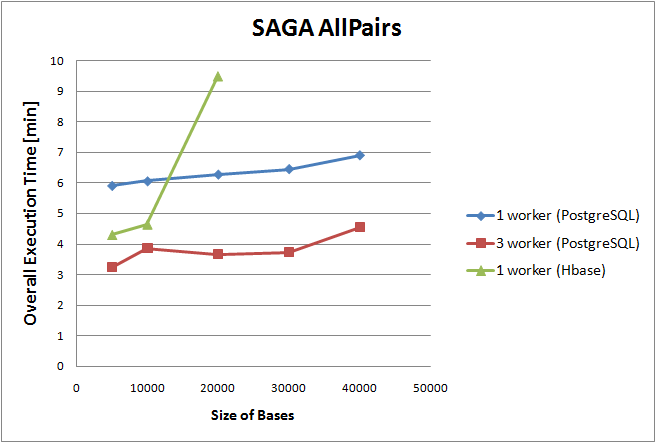
\includegraphics[width=0.8\textwidth]{saga_allpairs_1and3workers.png}
%           \caption{}
%       \label{saga_allpairs_1and3workers.png}
% \end{figure}

\jhanote{traditional algorithms are OK when data are limited.. but
  data requirements can change in different ways.. not only will data
  be greater, but also after a point will also be distributed. This is
  indicative of the data-gathering process (multiple-resources,
  replicated?) also indicative of the fact that often data-collection
  is growing greater than data-analysis (for example exabyte data last
  year).  Finally, with data-distributed, comes the following (at
  least challenges): do we move data-to-compute, or compute-to-data,
  is there a transition point, and can the same application be written
  to support both modes?}

\jhanote{From above, we need to write what has been traditionally
  non-distributed applications, in a distributed fashion. General
  philosophy on how we write distributed applications... One approach
  is to use infrastructure independent frameworks.}

\jhanote{Motivation for why this work is important. Applications
  are developed with specific infrastructure in mind. So in a
  way are limited by the infrastructure.. so whereas application
  can be often be written to scale, infrastructure doesn't
  always..}

\jhanote{This is a new way of developing applications using high-level
  abstractions. These high-level abstractions in turn ways to
  encode/support certain patterns, in this case data-parallel/access
  patterns. In turn the abstractions are infrastructure independent}.


\jhanote{Outline the work in this paper. New concept. Thus one
  important requirement is to determine how these
  i) how these patterns work for real scientific applications, \\
  ii) how well the general-implementations of these patterns work with
  respect to native implementations of these patterns \\
  iii) combination of i and ii, i.e. how well these applications
  behave when encoded using these high-level abstractions
  in comparison on general purpose infrastructure\\
  The aim is not to report better or even equivalent performance of
  these ``generalized applications compared to the native
  implementation of these application..}
